\documentclass[aspectratio=169,dvipsnames]{beamer}
\usepackage[utf8]{inputenc}
\usefonttheme{serif}
\usetheme{boxes}
\setbeamertemplate{frametitle}[default][center]
\setbeamersize{text margin right=20mm, text margin left=20mm} 
\addtobeamertemplate{frametitle}{\vskip1cm}{}
\setbeamertemplate{navigation symbols}{}
\setbeamertemplate{itemize item}[circle]
\setbeamercolor{alerted text}{fg=black}

%% absolute positioning
\usepackage[absolute,overlay]{textpos}
\usepackage{mathrsfs} % https://www.ctan.org/pkg/mathrsfs

\usepackage{fancyvrb}
\usepackage{xspace}
\usepackage{changepage}
\usepackage[version=0.96]{pgf}
\usepackage{tikz}

\newcommand<>{\highlight}[1]{{\alt#2{\colorbox#2{yellow}{#1}}{#1}}}


\usetikzlibrary{fit,positioning,shapes.geometric,calc,decorations.pathmorphing}
%Information to be included in the title page:
\title{\bf\LARGE Papers We Love \textcolor{gray}{Milano} \#4}
\subtitle{Partial Computation of Programs\\[5pt] (Futamura 1983)}
\author{Edoardo Vacchi}
% \institute{Overleaf}
\date{19th February 2020}

\renewcommand{\P}{\ensuremath{\mathcal{P}}\xspace}
\newcommand{\C}{\ensuremath{\mathcal{C}}\xspace}
\newcommand{\I}{\ensuremath{\mathcal{I}}\xspace}
\newcommand{\D}{\ensuremath{\mathcal{D}}\xspace}
\newcommand{\R}{\ensuremath{\mathcal{R}}\xspace}
 
\begin{document}
 
\frame{\titlepage}



\begin{frame}
    \centering
    
\includegraphics[width=\textwidth]{imgs/py1.png}
\end{frame}
    
\begin{frame}
    \textcolor<2>{lightgray}{
    The performance of many dynamic language implementations suffers 
    from high allocation rates and runtime type checks. This makes
    dynamic languages less applicable to purely algorithmic problems,
    despite their growing popularity. In this paper we present a simple
    \alert<2>{compiler optimization based on online partial evaluation} to remove
    object allocations and runtime type checks in the context of a tracing JIT. 
    We evaluate the optimization using a Python VM and find
    that it gives good results for all our (real-life) benchmarks.}

\end{frame}

\begin{frame}
    \tikz[overlay]
    \node at (6,-.5) {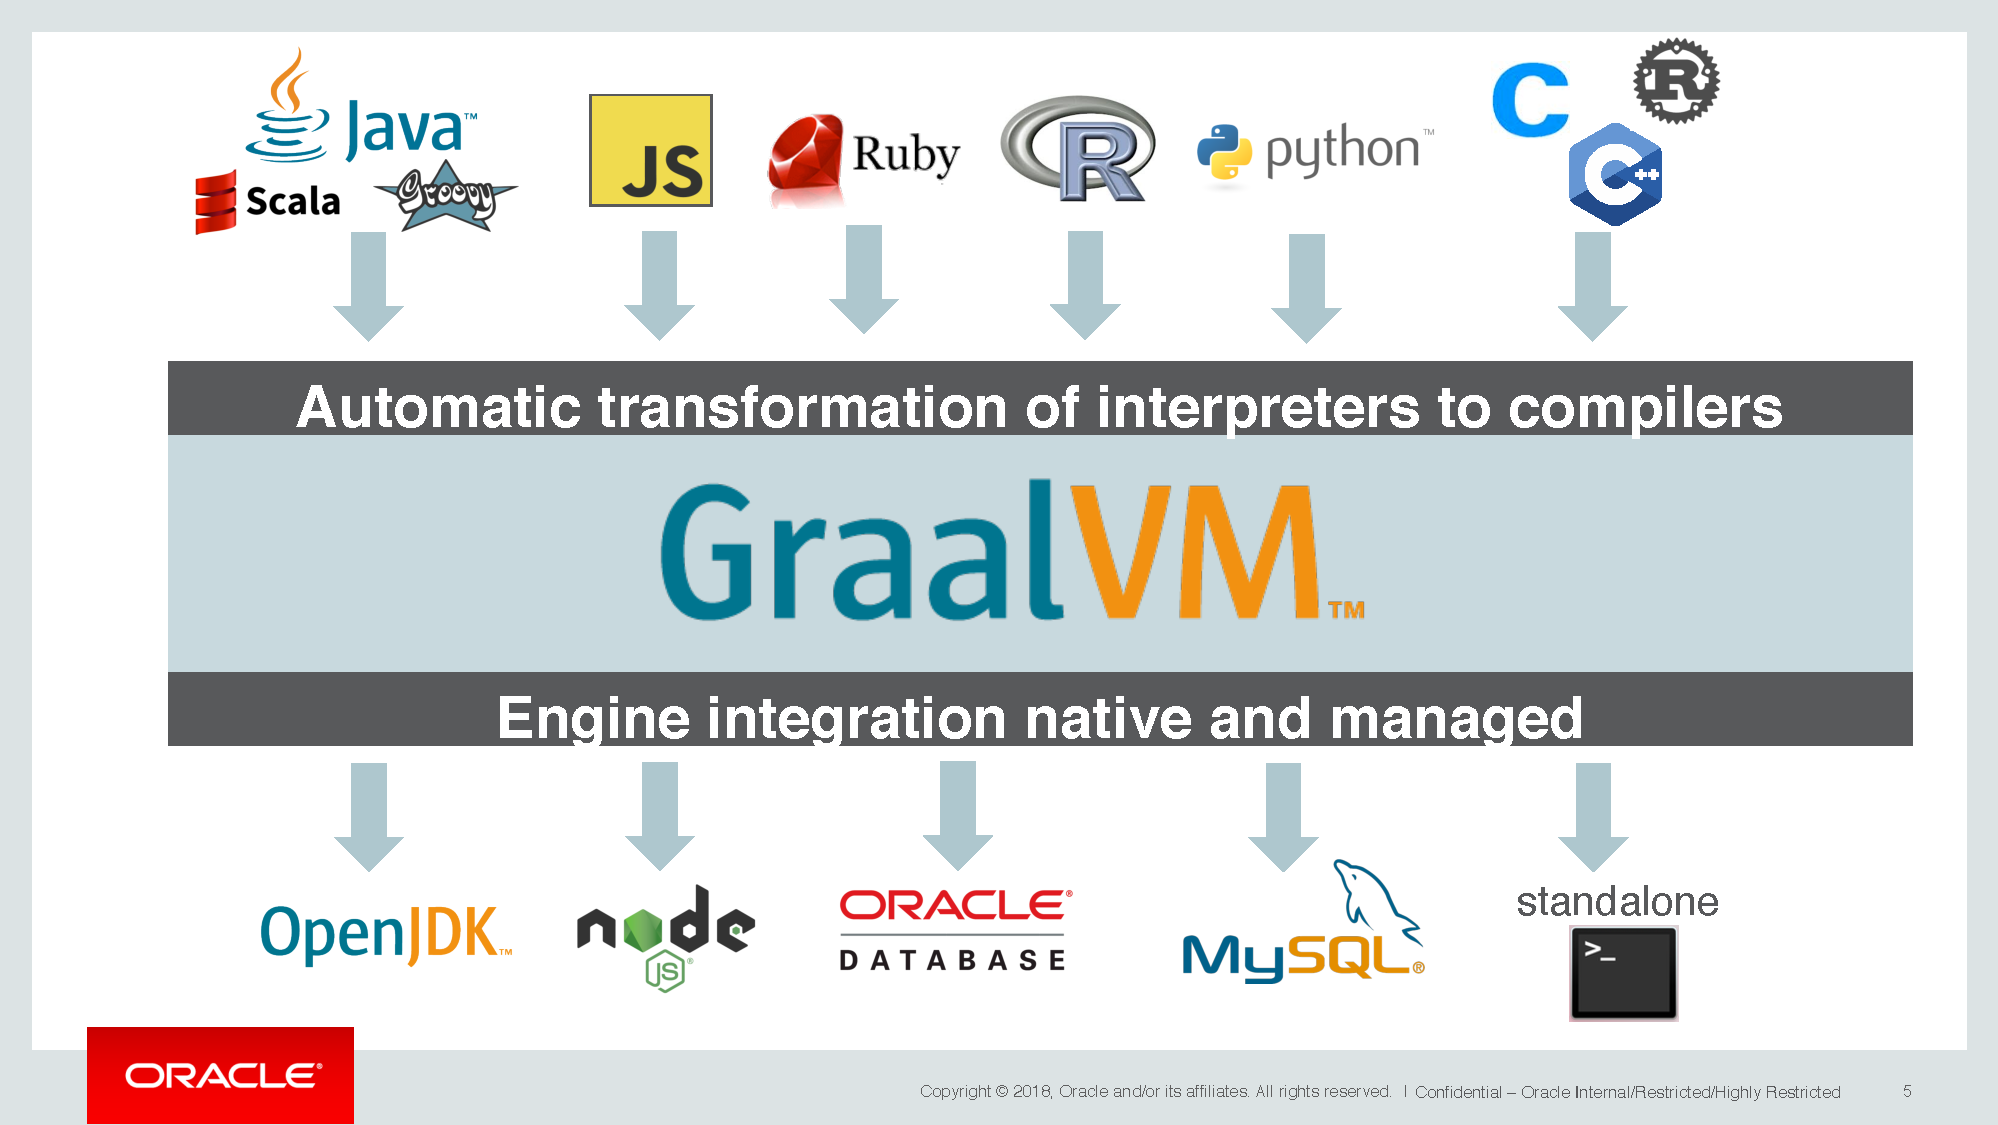
\includegraphics[width=15cm]{imgs/graalvm1.pdf}};
    \tikz[overlay]
    \node at (6,-5) {\footnotesize https://gotober.com/2018/sessions/650/graalvm-run-programs-faster-anywhere};
\end{frame}

\begin{frame}
    \tikz[overlay]
    \node at (6,-.5) {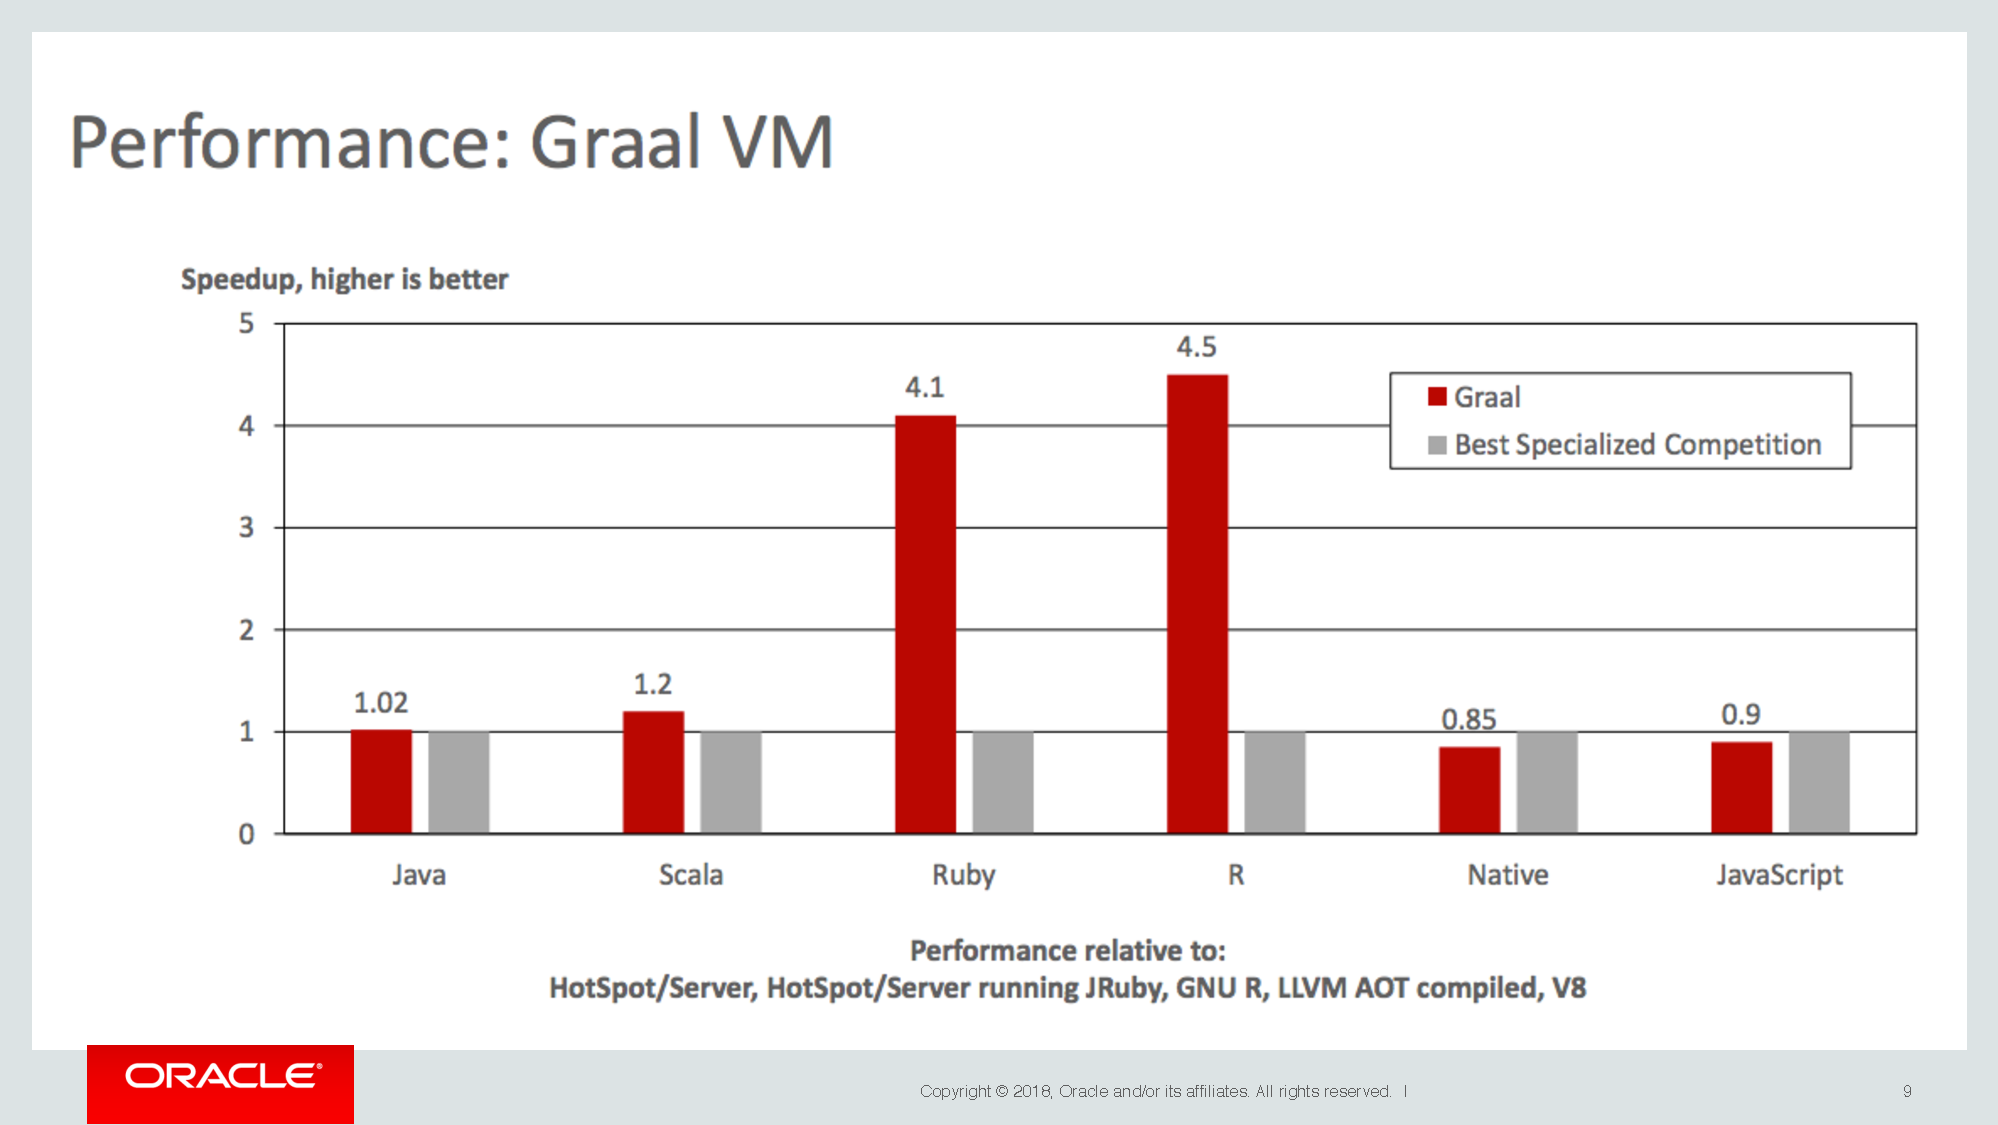
\includegraphics[width=15cm]{imgs/graalvm2.pdf}};
    \tikz[overlay]
    \node at (6,-5) {\footnotesize https://gotober.com/2018/sessions/650/graalvm-run-programs-faster-anywhere};
\end{frame}



\begin{frame}
    \centering
    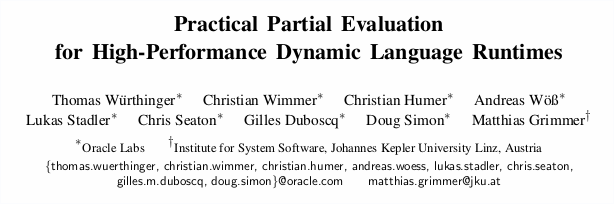
\includegraphics[width=\textwidth]{imgs/truffle.png}
\end{frame}
    

    \begin{frame}
\textcolor<2>{lightgray}{
        Most high-performance dynamic language virtual machines
\alert<2>{duplicate language semantics in the interpreter, compiler,
and runtime system}. This violates the principle to not repeat
yourself. In contrast, we define languages solely by \alert<2>{writing
an interpreter}. The interpreter performs specializations, e.g.,
augments the interpreted program with type information and
profiling information. Compiled code is derived automatically 
using \alert<2>{partial evaluation} while incorporating these specializations. 
\alert<2>{This makes partial evaluation practical in the
context of dynamic languages}: it reduces the size of the
compiled code while still compiling all parts of an operation
that are relevant for a particular program. When a speculation fails, 
execution transfers back to the interpreter, the program re-specializes 
in the interpreter, and later partial evaluation again transforms 
the new state of the interpreter to compiled code. 
}
% We evaluate our approach by comparing our
% implementations of JavaScript, Ruby, and R with best-in-class 
% specialized production implementations. Our general-purpose 
% compilation system is competitive with production
% systems even when they have been heavily optimized for the
% one language they support. For our set of benchmarks, our
% speedup relative to the V8 JavaScript VM is 0.83x, relative
% to JRuby is 3.8x, and relative to GNU R is 5x.
    \end{frame}


    \begin{frame}
        \textcolor<2>{lightgray}{\color<3>{white}
        We implement the language semantics only once in a
    simple form: as a \alert<2>{language interpreter} written in a 
    managed high-level host language.     \alert<2>{Optimized compiled code is
derived from the interpreter using partial evaluation}. This
    approach and its obvious benefits were described in 1971
    by Y. Futamura, and is known as the \textcolor<2->{red}{\textit{first Futamura
    projection}}. To the best of our knowledge no prior high-performance 
    language implementation used this approach.
        }
    \end{frame}
    

    

\begin{frame}
    \tikz[overlay]
    \node at (6,-.5) {
\includegraphics[width=19cm]{imgs/futamura.png}};
\end{frame}

\begin{frame}
    \centering
    \tikz 
    \node at (current page.center) {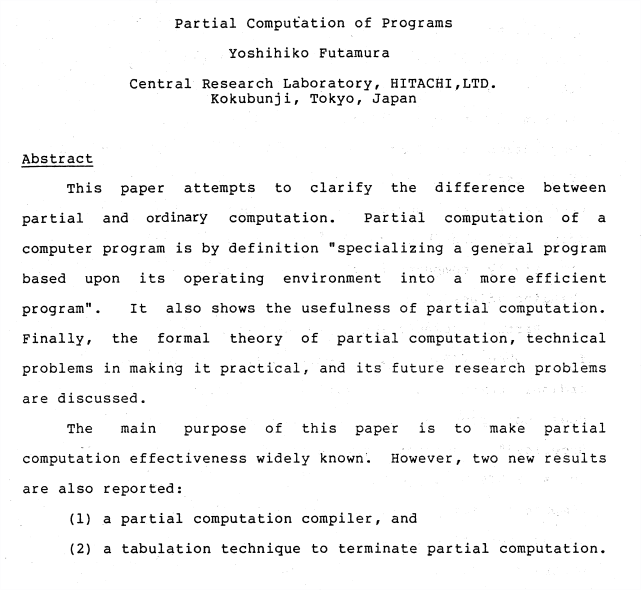
\includegraphics[width=.8\textwidth]{imgs/abstract.png}};
\end{frame}

\begin{frame}
    \centering
    \tikz 
    \node at (current page.center) {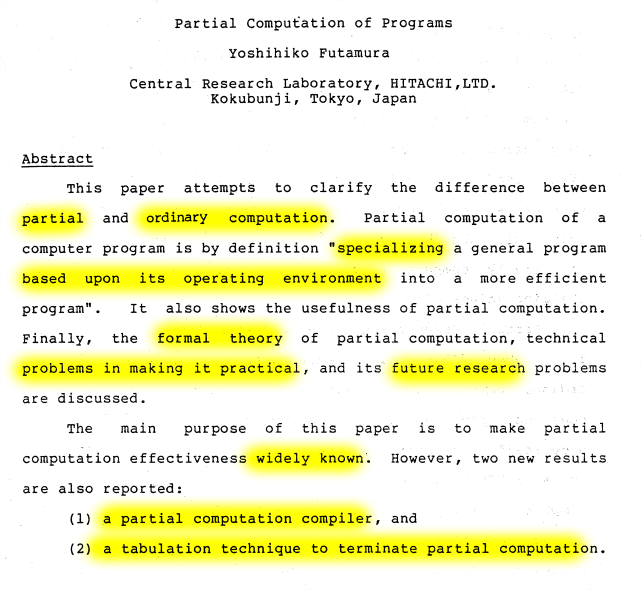
\includegraphics[width=.8\textwidth]{imgs/abstract-hl.png}};
\end{frame}

\begin{frame}
    \centering
    \tikz 
    \node at (current page.center) {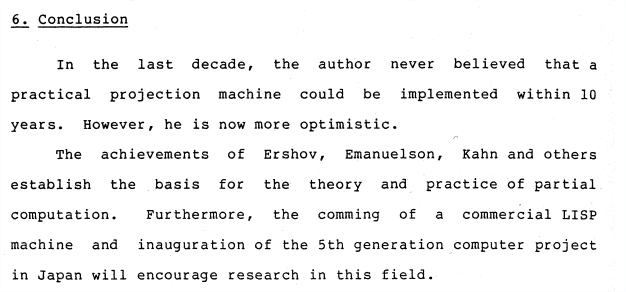
\includegraphics[width=.9\textwidth]{imgs/conclusions.png}};
\end{frame}

\begin{frame}    
    \centering
    \tikz 
    \node at (current page.center) {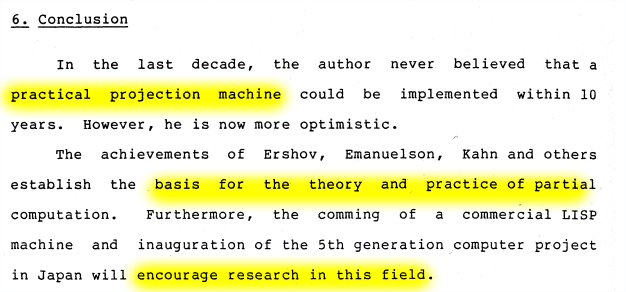
\includegraphics[width=.9\textwidth]{imgs/conclusions-hl.png}};
\end{frame}



\begin{frame}[c]
    \centering \Large \bf \color{Blue} Programs and Programming Languages 
    \end{frame}

\begin{frame}
    \tikz[overlay]
    \node[text width=.5\textwidth] at (1.3,-.5) {
    {\hspace{10pt}\Large \color{Blue} {Programs} }

    \begin{itemize}
        \item We call a \textit{program} a \textit{sequence of instructions}
         that can be \textit{executed} by a \textit{machine}.
         \item The \textit{machine} may be a \textit{virtual} machine or a \textit{physical} machine
        \item In the following, when we say that a \textit{program} is \textit{evaluated},
        we assume that there exists some \textit{machine} that is able to execute these instructions.
    \end{itemize}
    };
    \tikz[overlay]
    \node[text width=.5\textwidth] at (7.5,-.5) {
        
\includegraphics[width=10cm]{imgs/hackerman.jpg}
    };
\end{frame}

\begin{frame}{Program Evaluation}

    \begin{itemize}
        \item Consider a program \P, with input data \D;
        \item when we \textit{evaluate} \P over \D it produces
        some output result \R.
    \end{itemize}



    \begin{center}
    
        \begin{tikzpicture}
            \tikzstyle{every path}=[draw, ->]
            \tikzstyle{circ}=[draw, circle]
            \tikzstyle{box}=[draw, rectangle, text width=1cm, text height=.5cm, text centered, text depth=.3cm]
                \node [circ] (d) at (2,2) {\D};    
                \node [circ] (r) at (8,2) {\R};    
                \node [box] (p) at (5,2) {\P}; 
                \path (d) -- (p);    
                \path (p) -- (r);    
        \end{tikzpicture}
        
    \end{center}


    
\end{frame}

\begin{frame}

    \[
        f(k,u) = k+u
    \]

    \begin{center}
    
        \begin{tikzpicture}
            \tikzstyle{every path}=[draw, ->]
            \tikzstyle{circ}=[draw, circle, text centered]
            \tikzstyle{box}=[draw, rectangle, text width=1cm, text height=.5cm, text centered, text depth=.3cm]
                \node [circ, text width=1cm] (d) at (2,2) {$3,4$};    
                \node [circ, text width=1cm] (r) at (8,2) {$7$};    
                \node [box] (p) at (5,2) {$k+u$}; 
                \path (d) -- (p);    
                \path (p) -- (r);    
        \end{tikzpicture}
        
    \end{center}



\end{frame}

\begin{frame}{Interpreters}

    \begin{itemize}
    \item An \textit{interpreter} $\mathcal{I}$ is a \textit{program} 
    \item it \textit{evaluates} some other given program $\mathcal{P}$
    over some given data $\mathcal{D}$, and it produces the output
    result \R.
    \end{itemize}


\begin{center}

    \begin{tikzpicture}
        \tikzstyle{every path}=[draw, ->]
        \tikzstyle{circ}=[draw, circle]
        \tikzstyle{box}=[draw, rectangle, text width=1cm, text height=.5cm, text centered, text depth=.3cm]
            \node [circ] (p) at (2,3) {\P};    
            \node [circ] (d) at (2,1) {\D};    
            \node [circ] (r) at (8,2) {\R};    
            \node [box] (i) at (5,2) {\I}; 
            \path (p) -- (i);    
            \path (d) -- (i);    
            \path (i) -- (r);    
    \end{tikzpicture}
    
\end{center}


\begin{itemize}
    \item We denote this with $\I(\P,\D)$ 
\end{itemize}

\end{frame}

\begin{frame}\centering
    \begin{tikzpicture}
        \tikzstyle{every path}=[draw, ->]
        \tikzstyle{circ}=[draw, circle]
        \tikzstyle{box}=[inner sep=10pt, draw, rectangle, align=left]
        \node[text width=3cm] (p)  at (3,2) {
            $f(k,u) = k+u$
        };
        \node[text width=4cm] (p)  at (3,0) {
            \textbf{Instructions}

            \texttt{add x y}

            \texttt{sub x y}
            
            \texttt{mul x y}
            
            \texttt{...}
        };
        
        \node [inner sep=8pt, align=left] (i) at (10,0) {
            $\textbf{push}(\D)$\\
            $\textbf{while}(\textrm{true})$ \\

            $\quad \textrm{instr} \gets \textit{fetch-next}(\P)$ \\
            
            \quad \textbf{switch}({instr.op}): \\
            \quad \quad \textbf{case} \texttt{'add'}: \\
            \quad \quad \quad 
                $\texttt{x}\gets \textbf{pop}()$\\
            \quad \quad \quad 
                $\texttt{y}\gets \textbf{pop}()$ \\
                
            \quad \quad \quad 
                $\textrm{result} \gets x+y$ \\
            \quad \quad \quad 
                $\textbf{push}(\textrm{result})$ \\
            \quad \quad \textbf{case} \dots \\

        };
\end{tikzpicture}

\end{frame}



\begin{frame}{Compilers}

    \begin{itemize}

        \item 
            Let be \P a program that evaluates to \R when given \D;
        \item  
            A \textit{compiler} $\mathcal{C}$ translates a \textbf{source program}
            $\mathcal{P}$ into an \textbf{object program} $\C(\P)$ that
            evaluated over an input \D still produces \R
        
    
    
    \end{itemize}


    \begin{center}
    
        \begin{tikzpicture}
            \tikzstyle{every path}=[draw, ->]
            \tikzstyle{circ}=[draw, circle]
            \tikzstyle{box}=[draw, rectangle, text width=1cm, text height=.5cm, text centered, text depth=.3cm]
                \node [circ] (p)   at (2,2) {\P};    
                \node [box]  (c)   at (5,2) {\C}; 
                \node [circ] (cp)  at (8,2) {\tiny $\C(\P)$};    
                \node [box]  (cp2) at (5,0) {\small $\C(\P)$};    
                \node [circ] (d)   at (2,0) {\D};    
                \node [circ] (r)   at (8,0) {\R};    
                \path (p) -- (c);    
                \path (c) -- (cp);    
                \path (d) -- (cp2);    
                \path (cp2) -- (r);    
        \end{tikzpicture}
        
    \end{center}

\begin{itemize}
    \item We denote this with $\C(\P)(\D)$
\end{itemize}

\end{frame}

\begin{frame}[fragile,c]
    \begin{verbatim}
    sum:
        lea     eax, [rdi+rsi]
        ret
    \end{verbatim}
\end{frame}

\begin{frame}[fragile]
\tikz[overlay]
\node[text width=.5\textwidth] at (0,-3) {
    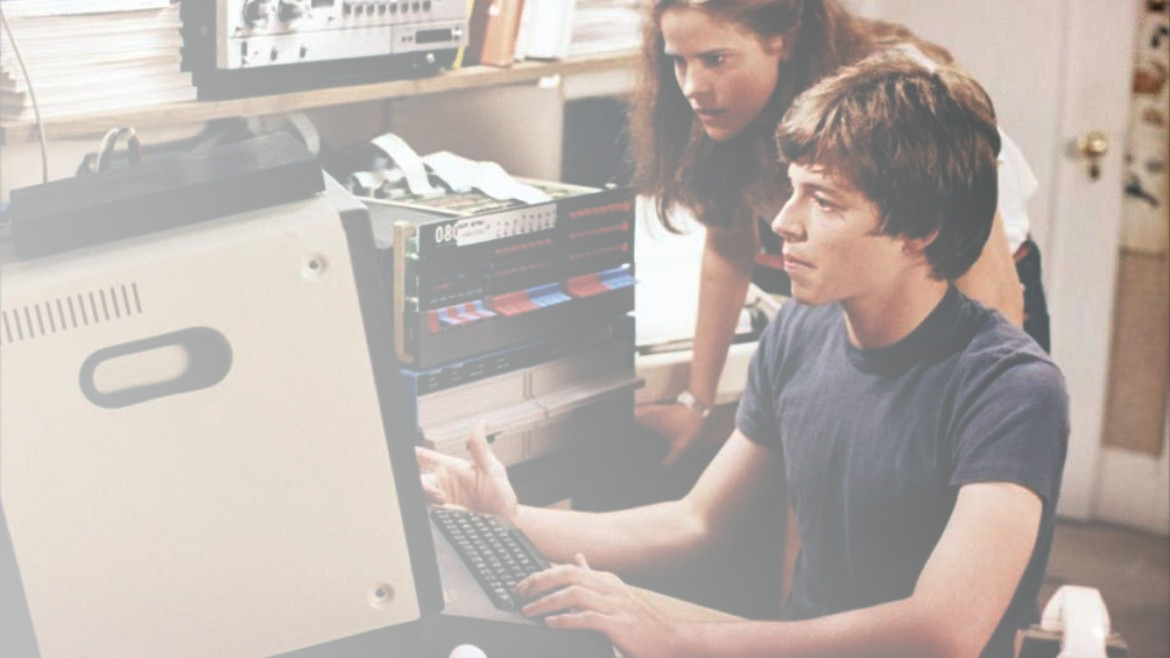
\includegraphics[width=18cm]{imgs/wargames-dimmed.jpg}
};
\begin{verbatim}
$ cat example.ml 
print_string "Hello world!\n"

$ ocaml example.ml 
Hello world!

$ ocamlc example.ml 

$ ./a.out 
Hello world!
\end{verbatim}
\end{frame}

% \begin{frame}
%     \begin{itemize}
%     \item \textit{With a bit of abuse of notation}, let us denote the result 
%     of a program \P evaluated over an input \D with \[
%         \P(\D)
%         \] 
%     \pause
%     \item Now, if we indicate $\P'$ with $\C(\P)$ we can write the following:
%     \end{itemize}
%     \begin{eqnarray*}        
%         \P(\D) &=& \R\\
%         \C(\P) &=& \P'\\
%         \P'(\D) &=& \R\\
%         \C(\P)(\D) &=& \R\\
%         \I(\P, \D) &=& \R\\
%         \C(\P)(\D) &=& \I(\P, \D) \\
%     \end{eqnarray*}
    
% \end{frame}

\begin{frame}[c]

    \begin{center}
        \Large \[
            \C(\P)(\D) = \I(\P, \D) 
        \]
    \end{center}

\end{frame}


\begin{frame}[c]
    \centering \Large \bf \color{Blue} Partial Evaluation 
\end{frame}

\begin{frame}{Partial Evaluation (intuition)}
\begin{center}Let us have a computation $f$ of two parameters $k$, $u$\end{center}
    \[
        f(k,u)
    \]
    \begin{itemize}
    \item Now suppose that $f$ is often called with $k=5$; 
    
    \item we may define the program $f_5(u)$ by substituting $5$ for $k$ in $f$ 
    and doing all possible computation based upon value $5$.

    \item  Partial evaluation is the process of rewriting $f(5,u)$ into $f_5(u)$
    \end{itemize}
\end{frame}
 


\begin{frame}

    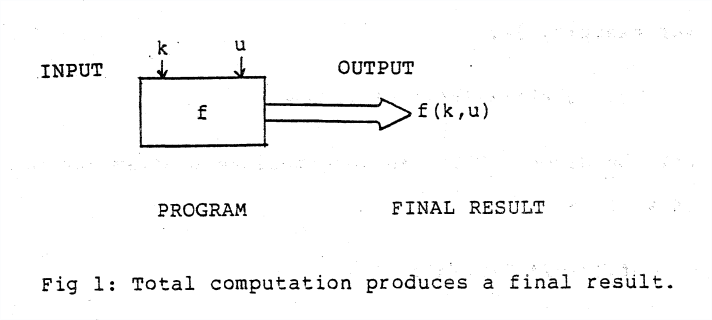
\includegraphics[width=\textwidth]{imgs/fig1.png}

\end{frame}
 


\begin{frame}

    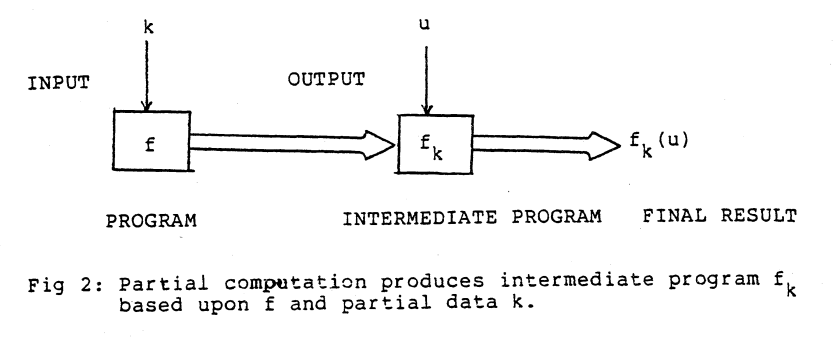
\includegraphics[width=\textwidth]{imgs/fig2.png}

\end{frame}




\begin{frame}[fragile]
\begin{adjustwidth}{-3em}{-4em}
\tikz[remember picture, overlay] 
\node at (17,-4) {
\includegraphics[height=10cm]{imgs/unix.jpg}};

{ \Large\color{Blue}{This is Currying! I Know This!}}

\begin{minipage}{0.50\textwidth}
\vspace{15pt}
\begin{itemize}
    \item Not exactly!
        In \emph{functional programming} \emph{currying} or 
        \emph{partial application} is $f_5(u) := f(5,u)$

\begin{verbatim}
let f = 
 (k, u) =>  
  k * (k * (k+1) + u + 1) + u * u;
let f5 = (u) => f(5, u);
\end{verbatim}
\item In a functional programming language this usually \emph{does not change}
            the program that implements $f$
\end{itemize}


\end{minipage}
\end{adjustwidth}
\end{frame}

\begin{frame}[fragile]{Simplification}

\begin{center}

\texttt{let f = (k, u) => k * (k * (k+1) + u + 1) + u * u;} \\[10pt]

by fixing $k=5$ and \textit{simplifying}: \\[10pt]

\texttt{let f5 = (u) => 5 * (31 + u) + u * u;} \\[10pt]

% because $f(2,u) = f_2(u)$ for any value of $u$, 

\end{center}

\end{frame}


\begin{frame}[fragile]{Rewriting}
    \begin{verbatim}
        function pow(n, k) {
            if (k <= 0) {
                return 1;
            } else {
                return n * pow(n, k-1);
            }
        }
        function pow5(n) {
            return pow(n, 5);
        }
    \end{verbatim}
    \tikz[remember picture, overlay] 
    \node[anchor=west,color=yellow,fill=yellow,draw,rectangle,text width=1.7cm, text height=.2cm, opacity=.5] 
            at (3.7,2) {};
\end{frame}

\begin{frame}[fragile]{Rewriting}
    \begin{verbatim}
        function pow(n, k) {
            if (k <= 0) {
                return 1;
            } else {
                return n * pow(n, k-1);
            }
        }
        function pow5(n) {
            return n * pow(n, 4);
        }
    \end{verbatim}
    \tikz[remember picture, overlay] 
    \node[anchor=west,color=yellow,fill=yellow,draw,rectangle,text width=2.5cm, text height=.2cm, opacity=.5] 
    at (3.7,2) {};
\end{frame}

\begin{frame}[fragile]{Rewriting}
    \begin{verbatim}
        function pow(n, k) {
            if (k <= 0) {
                return 1;
            } else {
                return n * pow(n, k-1);
            }
        }
        function pow5(n) {
            return n * n * pow(n, 3);
        }
    \end{verbatim}
    \tikz[remember picture, overlay] 
    \node[anchor=west,color=yellow,fill=yellow,draw,rectangle,text width=3.5cm, text height=.2cm, opacity=.5] 
    at (3.7,2) {};
\end{frame}

\begin{frame}[fragile]{Rewriting}
    \begin{verbatim}
        function pow(n, k) {
            if (k <= 0) {
                return 1;
            } else {
                return n * pow(n, k-1);
            }
        }
        function pow5(n) {
            return n * n * n * n * n;
        }
    \end{verbatim}
\tikz[remember picture, overlay] 
\node[anchor=west,color=yellow,fill=yellow,draw,rectangle,text width=3.5cm, text height=.2cm, opacity=.5] 
at (3.7,2) {};
\end{frame}



\begin{frame}[fragile]{Rewriting}
    \begin{verbatim}
        function pow(n, k) {
            if (k <= 0) {
                return 1;
            } else {
                return n * pow(n, k-1);
            }
        }
        function pow5(n) {
            return n * n * n * n * n;
        }
    \end{verbatim}
\tikz[remember picture, overlay] 
\node[anchor=west,color=yellow,fill=yellow,draw,rectangle,text width=3.5cm, text height=.2cm, opacity=.5] 
at (3.7,2) {};

\centering 
In compiler implementation this is sometimes called \textit{inlining}

\end{frame}


\begin{frame}{Rewriting and Simplification}
    \begin{itemize}
    % \item In a \textit{recursive program schema} 
    % (\textit{e.g.,} lambda calculus, partial recursive functions) 
    % these are called \textit{rewriting} and \textit{simplification}.

    \item \textbf{Rewriting} is
    similar to macro expansion and \textit{procedure integration} 
    (\textit{$\beta$-reduction}, \textit{inlining})
    in the optimization technique of a compiler.
    
    \item    Often combined with
    \textbf{simplification} (\textit{constant folding})

    \end{itemize}

    \centering
    \tikz 
    \node at (current page.center) {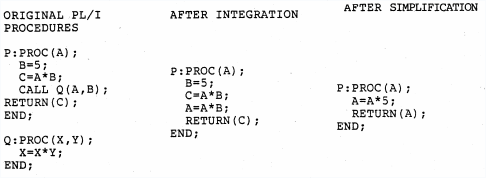
\includegraphics[width=.7\textwidth]{imgs/fig6.png}};

    
\end{frame}


\begin{frame}{Projection}
\centering 
    The following equation holds for $f_k$ and $f$
    \begin{equation}
        f_k(u)=f(k,u)
    \end{equation}

we call $f_k$ \textit{a projection of $f$ at $k$}
\end{frame}

\begin{frame}{Partial Evaluator}

    A partial computation procedure may be a computer program $\alpha$
    called \textit{a projection machine}, \textit{partial computer} 
    or \textit{partial evaluator}.
    
    \begin{equation}
        \alpha(f,k) = f_k
    \end{equation}
    
\end{frame}


\begin{frame}{Partial Evaluator}
    
\begin{center}

    \begin{tikzpicture}
        \tikzstyle{every path}=[draw, ->]
        \tikzstyle{envel}=[shape=ellipse, draw]
        \tikzstyle{circ}=[draw, circle]
        \tikzstyle{box}=[draw, rectangle, text width=1cm, text height=.5cm, text centered, text depth=.3cm]
            \node [circ] (in1) at (2,3) {$k$};    
            \node [circ] (in2) at (2,1) {$u$};    
            \node [circ] (out) at (8,2) {$f(k,u)$};    
            \node [box] (box) at (5,2) {$f$};
            
            
            \path (in1) -- (box);    
            \path (in2) -- (box);    
            \path (box) -- (out);

            \pause

            \begin{scope}[shift={(in1))},x={(box)},y={($(in1)!1!90:(box)$)}]
                \draw[red] (.5,0) ellipse (.8 and .5);
            \end{scope}

            \pause

            \node[box](proj) at (5,-.5) {$f_k$};

            \draw[
                line join=round,
                decorate, decoration={
                zigzag,
                segment length=4,
                amplitude=1,post=lineto,
                post length=2pt}] (5,.9) -- (proj) node [midway, label=right:{$\alpha$}] {} ;
            
    \end{tikzpicture}
    
\end{center}

\end{frame}




\begin{frame}[fragile]{Partial Evaluator}
    \begin{verbatim}
        function pow(n, k) {
            if (k <= 0) {
                return 1;
            } else {
                return n * pow(n, k-1);
            }
        }
        let pow5 = alpha(pow, {k:5});
        // (n) => n * n * n * n * n;
    \end{verbatim}
    \tikz[remember picture, overlay] 
\node[anchor=west,color=yellow,fill=yellow,draw,rectangle,text width=3.5cm, text height=.2cm, opacity=.5] 
at (3.7,2) {};
\end{frame}



% \begin{frame}{Basic Equation of Partial Evaluation}

%     $\alpha$ is a partial evaluator; but $\alpha$ is itself a program.

%     Thus, consider $\alpha_f$, the partial evaluation of $\alpha$ at $f$:
% \begin{eqnarray}
%             \alpha_f(k) &=& \alpha(f,k) \nonumber \\
%             \alpha(f,k) &=& f_k         \nonumber \\
%             \alpha_f(k) &=& f_k 
% \end{eqnarray}

% \end{frame}

\setcounter{equation}{3}

\setbeamercovered{transparent} 

\begin{frame}{Examples}

    The paper presents:

    \begin{itemize}
        \item<1> Automatic theorem proving
        \item<1> Pattern matching
        \item<1> Syntax analyzer
        \item<1,2> Automatically generating a compiler
    \end{itemize}
    
\end{frame}

\setbeamercovered{} 

\begin{frame}{Interpreters and Compilers (\textit{reprise})}
    \begin{itemize}
        \item An interpreter is a \textit{program}
        \item This \emph{program} takes another \textit{program} and the data as input
        \item It evaluates the program on the input and returns the result

    \end{itemize}
    \[
        \I(\P,\D) %= \R    
    \]

    \begin{itemize}
        \item A compiler is a \textit{program}
        \item This \emph{program} takes a \textit{source program} 
                and returns an \textit{object program}
        \item The \textit{object program} processes the input and returns the result
    \end{itemize}
    \[
        \C(\P)(\D) %= \R    
    \]

\end{frame}



\begin{frame}{Partial Evaluation of an Interpreter}


\begin{center}

    \begin{tikzpicture}
        \tikzstyle{every path}=[draw, ->]
        \tikzstyle{envel}=[shape=ellipse, draw]
        \tikzstyle{circ}=[draw, circle]
        \tikzstyle{box}=[draw, rectangle, text width=1cm, text height=.5cm, text centered, text depth=.3cm]
            \node [circ] (in1) at (2,3) {\P};    
            \node [circ] (in2) at (2,1) {\D};    
            \node [circ] (out) at (8,2) {\R};    
            \node [box] (box) at (5,2) {\I};
            
            
            \path (in1) -- (box);    
            \path (in2) -- (box);    
            \path (box) -- (out);

            \pause

            \begin{scope}[shift={(in1))},x={(box)},y={($(in1)!1!90:(box)$)}]
                \draw[red] (.5,0) ellipse (.8 and .5);
            \end{scope}

            \pause

            \node[box](proj) at (5,-.5) {$\I_\P$};

            \draw[
                line join=round,
                decorate, decoration={
                zigzag,
                segment length=4,
                amplitude=1,post=lineto,
                post length=2pt}] (5,.9) -- (proj) node [midway, label=right:{$\alpha$}] {} ;
            
    \end{tikzpicture}
    
\end{center}

\end{frame}


\begin{frame}{Partially Evaluated Interpreter}
    \begin{center}
    
        \begin{tikzpicture}
            \tikzstyle{every path}=[draw, ->]
            \tikzstyle{circ}=[draw, circle]
            \tikzstyle{box}=[draw, rectangle, text width=1cm, text height=.5cm, text centered, text depth=.3cm]
                \node [circ] (in) at (2,2) {\D};    
                \node [circ] (out) at (8,2) {\R};    
                \node [box] (box) at (5,2) {$\I_\P$}; 
                \path (in) -- (box);    
                \path (box) -- (out);    
        \end{tikzpicture}
        
    \end{center}

    \begin{itemize}
    \item That is, by feeding \D into $\I_\P$, you get \R;
    \item in other words, $\I_\P$ is \textit{an object program}.
    \end{itemize}
    
\end{frame}


\begin{frame}{First Equation of Partial Computation (First Projection)}

    
% An \textit{interpreter} $\mathcal{I}$ is a program to perform
% specified computations that analyze the meanings of a given program, 
% say $\mathcal{P}$, based upon given data, say $\mathcal{D}$. 

We recall the previous definitions of \textit{interpreter}
and \textit{compiler}.

\begin{eqnarray}
    \mathcal{I}(\mathcal{P},\mathcal{D}) &=& \mathcal{C}(\mathcal{P})(\mathcal{D}) \nonumber \\
    \alpha(\mathcal{I},\mathcal{P}) &=& \mathcal{I}_{\mathcal{P}} \nonumber   \\ 
    \mathcal{I}_{\mathcal{P}} &=&  \mathcal{C}(\mathcal{P})
\end{eqnarray}


\end{frame}

\begin{frame}

            $\textbf{push}(\D)$\\
            \textcolor<2->{white}{$\textbf{while}(\textrm{true})$} \\

            \textcolor<2->{white}{$\quad \textrm{instr} \gets \textit{fetch-next}(\P)$} \\
            
            \textcolor<2->{white}{\quad \textbf{switch}({instr.op})}: \\
            \quad \quad \textbf{case} \texttt{'add'}: \\
            \quad \quad \quad 
                $\texttt{x}\gets \textbf{pop}()$\\
            \quad \quad \quad 
                $\texttt{y}\gets \textbf{pop}()$ \\
                
            \quad \quad \quad 
                $\textrm{result} \gets x+y$ \\
            \quad \quad \quad 
                $\textbf{push}(\textrm{result})$ \\
            \textcolor<2->{white}{\quad \quad \textbf{case} \dots} \\


\end{frame}



\begin{frame}[fragile,c]
    \begin{verbatim}
    sum:
        lea     eax, [rdi+rsi]
        ret
    \end{verbatim}
\end{frame}

\begin{frame}{Partial Evaluation of an Interpreter}

\begin{center}

    \begin{tikzpicture}
        \tikzstyle{every path}=[draw, ->]
        \tikzstyle{envel}=[shape=ellipse, draw]
        \tikzstyle{circ}=[draw, circle]
        \tikzstyle{box}=[draw, rectangle, text width=1cm, text height=.5cm, text centered, text depth=.3cm]
            \node [circ] (in1) at (2,3) {\P};    
            \node [circ] (in2) at (2,1) {\D};    
            \node [circ] (out) at (8,2) {\R};    
            \node [box] (box) at (5,2) {\I};
            
            
            \path (in1) -- (box);    
            \path (in2) -- (box);    
            \path (box) -- (out);


            \begin{scope}[shift={(in1))},x={(box)},y={($(in1)!1!90:(box)$)}]
                \draw[red] (.5,0) ellipse (.8 and .5);
            \end{scope}

            \node[box](proj) at (5,-.5) {$\I_\P$};

            \draw[
                line join=round,
                decorate, decoration={
                zigzag,
                segment length=4,
                amplitude=1,post=lineto,
                post length=2pt}] (5,.9) -- (proj) node [midway, label=right:{$\alpha$}] {} ;
            
    \end{tikzpicture}
    
\end{center}

\end{frame}

\begin{frame}{\uncover<2>{Partial Evaluation of the } \\ Partial Evaluation of an Interpreter}

    \begin{center}
    
        \begin{tikzpicture}
            \tikzstyle{every path}=[draw, ->]
            \tikzstyle{envel}=[shape=ellipse, draw]
            \tikzstyle{circ}=[draw, circle]
            \tikzstyle{box}=[draw, rectangle, text width=1cm, text height=.5cm, text centered, text depth=.3cm]
                \node [circ] (in1) at (2,3) {\I};    
                \node [circ] (in2) at (2,1) {\P};    
                \node [circ] (out) at (8,2) {$\I_\P$};    
                \node [box] (box) at (5,2) {$\alpha$};
                
                
                \path (in1) -- (box);    
                \path (in2) -- (box);    
                \path (box) -- (out);
    
                \pause
    
                \begin{scope}[shift={(in1))},x={(box)},y={($(in1)!1!90:(box)$)}]
                    \draw[red] (.5,0) ellipse (.8 and .5);
                \end{scope}
    
                \pause
    
                \node[box](proj) at (5,-.5) {$\alpha_\I$};
    
                \draw[
                    line join=round,
                    decorate, decoration={
                    zigzag,
                    segment length=4,
                    amplitude=1,post=lineto,
                    post length=2pt}] (5,.9) -- (proj) node [midway, label=right:{$\alpha$}] {} ;
                
        \end{tikzpicture}
        
    \end{center}
    
    \end{frame}


    

\begin{frame}{Second Equation of Partial Computation (Second Projection)}

    

    \begin{center}
    
        \begin{tikzpicture}
            \tikzstyle{every path}=[draw, ->]
            \tikzstyle{circ}=[draw, circle]
            \tikzstyle{box}=[draw, rectangle, text width=1cm, text height=.5cm, text centered, text depth=.3cm]
                \node [circ] (in) at (2,2) {\P};    
                \node [circ] (out) at (8,2) {$\only<1>{\I_\P}\only<2->{\C(\P)}$};    
                \node [box] (box) at (5,2) {$\only<1-3>{\alpha_\I}\only<4>{\C}$}; 
                \path (in) -- (box);    
                \path (box) -- (out);    
        \end{tikzpicture}
        
    \end{center}


    \begin{equation}
    \alpha_\mathcal{I}(\mathcal{P}) =  \mathcal{I}_\mathcal{P}
    \end{equation}
    
    \begin{itemize}
        \item but $\I_\P$, evaluated on \D gives \R 
        \item<2-> then $\I_\P$ is an object program ($\P'=\C(\P)$)
        \item<3-> $\alpha_\I$ transforms a source program $\P$ to $\I_\P$ (\textit{i.e.,} $\C(\P)$)
        \item<4-> then $\alpha_\I$ is \textit{a compiler}
    \end{itemize}
    
\end{frame}


\begin{frame}
    \tikz[overlay]
    \node at (5,0) {
\includegraphics[width=19cm]{imgs/inception.jpg}};
\end{frame}


\begin{frame}{Partial Evaluation of the \\Partial Evaluation of an Interpreter}

    \begin{center}
    
        \begin{tikzpicture}
            \tikzstyle{every path}=[draw, ->]
            \tikzstyle{envel}=[shape=ellipse, draw]
            \tikzstyle{circ}=[draw, circle]
            \tikzstyle{box}=[draw, rectangle, text width=1cm, text height=.5cm, text centered, text depth=.3cm]
                \node [circ] (in1) at (2,3) {\I};    
                \node [circ] (in2) at (2,1) {\P};    
                \node [circ] (out) at (8,2) {$\I_\P$};    
                \node [box] (box) at (5,2) {$\alpha$};
                
                
                \path (in1) -- (box);    
                \path (in2) -- (box);    
                \path (box) -- (out);
    
    
                \begin{scope}[shift={(in1))},x={(box)},y={($(in1)!1!90:(box)$)}]
                    \draw[red] (.5,0) ellipse (.8 and .5);
                \end{scope}
    
    
                \node[box, text width=2cm](proj) at (5,-.5) {$\alpha_\I=\C$};
    
                \draw[
                    line join=round,
                    decorate, decoration={
                    zigzag,
                    segment length=4,
                    amplitude=1,post=lineto,
                    post length=2pt}] (5,.9) -- (proj) node [midway, label=right:{$\alpha$}] {} ;
                
        \end{tikzpicture}
        
    \end{center}
    
    \end{frame}


\begin{frame}{\uncover<3->{Partial Evaluation of the \\} Partial Evaluation of the \\ Partial Evaluation of an Interpreter}


    \begin{center}
    
        \begin{tikzpicture}
            \tikzstyle{every path}=[draw, ->]
            \tikzstyle{envel}=[shape=ellipse, draw]
            \tikzstyle{circ}=[draw, circle]
            \tikzstyle{box}=[draw, rectangle, text width=1cm, text height=.5cm, text centered, text depth=.3cm]
                \node [circ] (in1) at (2,3) {$\alpha$};    
                \node [circ] (in2) at (2,1) {\I};    
                \node [circ] (out) at (8,2) {$\alpha_\I=\C$};    
                \node [box] (box) at (5,2) {$\alpha$};
                
                
                \path (in1) -- (box);    
                \path (in2) -- (box);    
                \path (box) -- (out);
    
                \pause
    
                \begin{scope}[shift={(in1))},x={(box)},y={($(in1)!1!90:(box)$)}]
                    \draw[red] (.5,0) ellipse (.8 and .5);
                \end{scope}
    
                \pause
    
                \node[box](proj) at (5,-.5) {$\alpha_\alpha$};
    
                \draw[
                    line join=round,
                    decorate, decoration={
                    zigzag,
                    segment length=4,
                    amplitude=1,post=lineto,
                    post length=2pt}] (5,.9) -- (proj) node [midway, label=right:{$\alpha$}] {} ;
                
        \end{tikzpicture}
        
    \end{center}
    
    \end{frame}


\begin{frame}{Third Equation of Partial Computation (Third Projection)}

    \begin{center}
    
        \begin{tikzpicture}
            \tikzstyle{every path}=[draw, ->]
            \tikzstyle{circ}=[draw, circle]
            \tikzstyle{box}=[draw, rectangle, text width=1cm, text height=.5cm, text centered, text depth=.3cm]
                \node [circ] (in) at (2,2) {\I};    
                \node [circ] (out) at (8,2) {$\alpha_\I=\C$};    
                \node [box] (box) at (5,2) {$\alpha_\alpha$}; 
                \path (in) -- (box);    
                \path (box) -- (out);    
        \end{tikzpicture}
        
    \end{center}

    \begin{equation}
    \alpha_\alpha(\mathcal{I}) =  \alpha_\mathcal{I}
    \end{equation}
    
    \begin{itemize}
     \item $\alpha_\alpha$ is a program that given \I, returns $\alpha_\I=\C$
     \item $\alpha_\I$ transforms a source program to an object program
     \item $\alpha_\I$ is a compiler
     \item $\alpha_\alpha$ is a \textit{compiler-compiler} (a \textit{compiler generator})
            which generates a compiler $\alpha_\I$ from an interpreter $\I$
    \end{itemize}
\end{frame}

\begin{frame}
    \centering
    \tikz
    \node at (0,0) {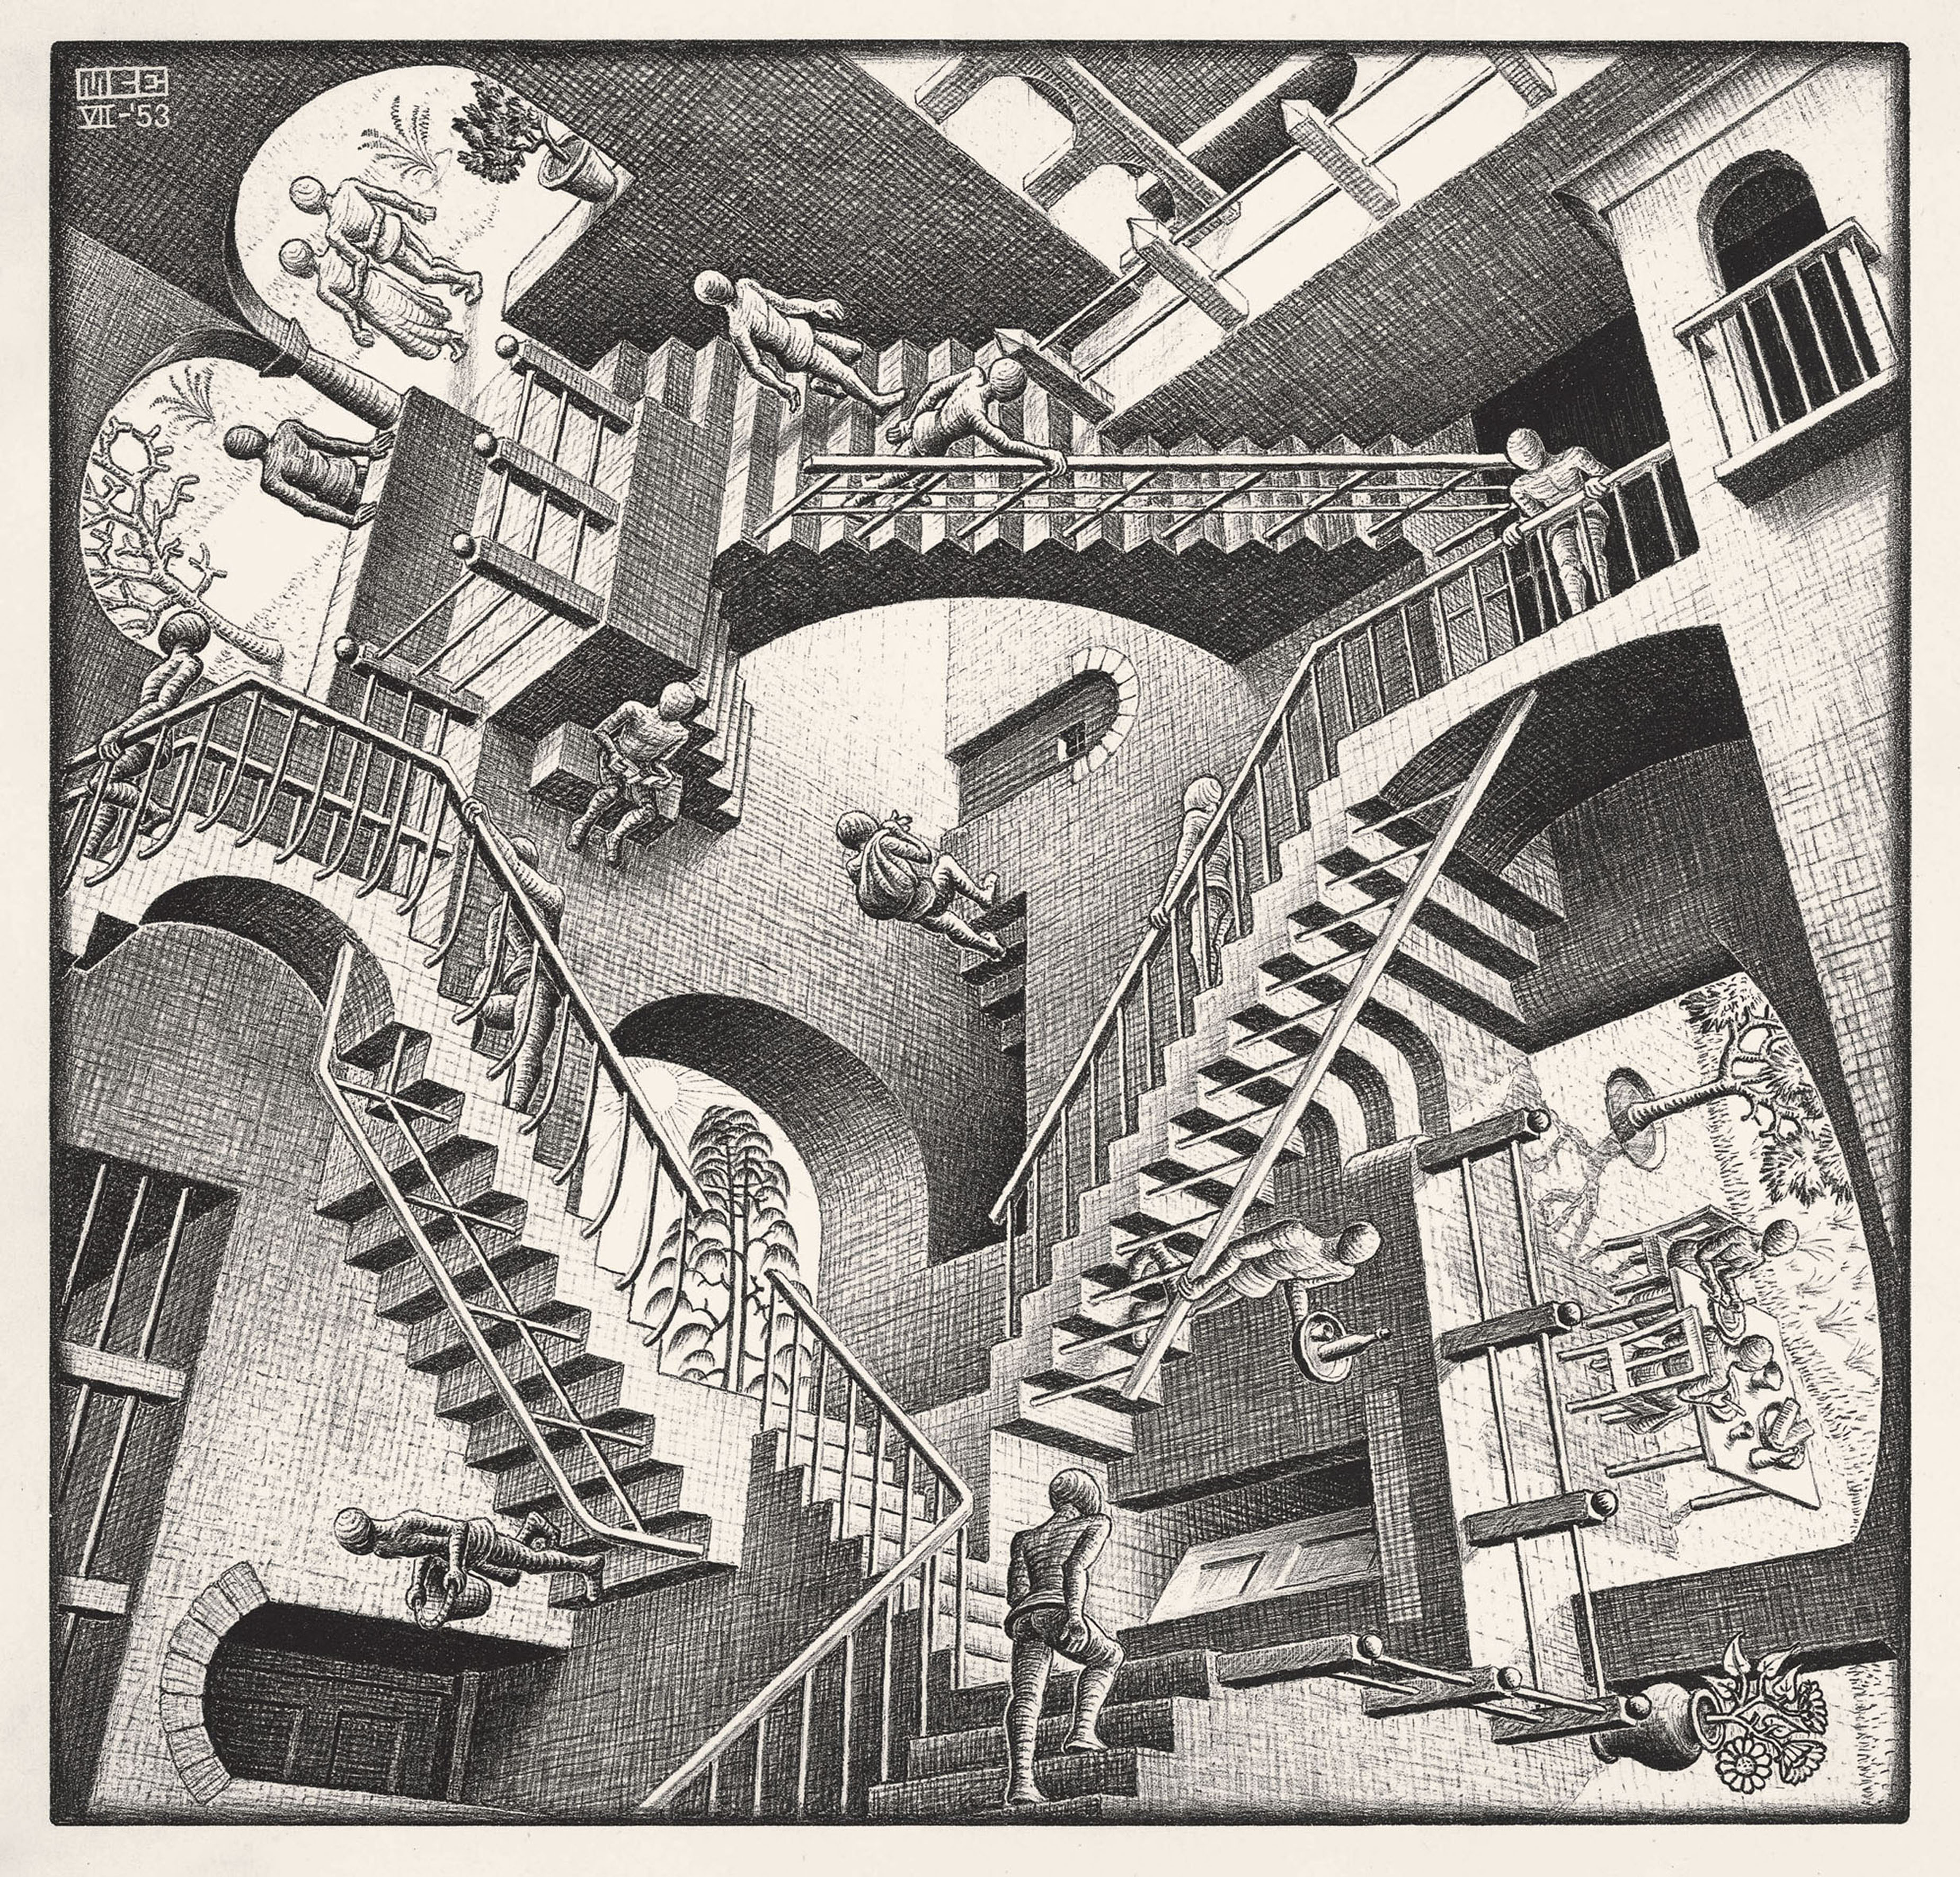
\includegraphics[width=9cm]{imgs/escher.jpg}};
\end{frame}


\begin{frame}{Partial Evaluation of a Partially-Evaluated Evaluator}

    \begin{itemize}
    \item Let us call \textbf{\I-language} a language implemented by interpreter \I,  
    
    \[
        \alpha_\alpha(\mathcal{I}) =  \alpha_\mathcal{I}
    \]
    

    \item $\alpha_\I$ is then a \textbf{\I-language compiler}
    
    \item let us now substitute $\alpha$ for $\I$ in $\alpha_\alpha(\mathcal{I}) = \alpha_\mathcal{I}$,
    \item which means considering $\alpha$ an interpreter for the $\alpha$-language.
    
    \[
        \alpha_\alpha(\alpha)=\alpha_\alpha    
    \]

    \item $\alpha_\alpha$ is an \textbf{$\alpha$-language} compiler.


    \end{itemize}


\end{frame}

\begin{frame}{Fourth Equation of Partial Computation}

    \[
        \alpha_\alpha(\alpha)=\alpha_\alpha    
    \]

    \begin{center}
    
        \begin{tikzpicture}
            \tikzstyle{every path}=[draw, ->]
            \tikzstyle{circ}=[draw, circle]
            \tikzstyle{box}=[draw, rectangle, text width=1cm, text height=.5cm, text centered, text depth=.3cm]
                \node [circ] (in) at (2,2) {$\alpha$};    
                \node [circ] (out) at (8,2) {$\alpha_\alpha$};    
                \node [box] (box) at (5,2) {$\alpha_\alpha$}; 
                \path (in) -- (box);    
                \path (box) -- (out);    
        \end{tikzpicture}
        
    \end{center}
    


    \begin{itemize}
    \item $\alpha_\alpha$ is an $\alpha$-language compiler.
    \item $\alpha_\alpha(\I)=\alpha_\I$ is an object program of $\I$; thus:
    \item What is the $\alpha$-language?
    \begin{equation}
        \alpha_\alpha(\I)(\P) =  \I_\P
    \end{equation}
    \end{itemize}


\end{frame}

\begin{frame}

    \begin{itemize}
        \item What is the $\alpha$-language?
        \begin{eqnarray*}
            \alpha_\alpha(\I)(\P) &=&  \I_\P \\
            \alpha_\alpha(f)(k)   &=&  f_k
        \end{eqnarray*}

    \item In other words, by finding $\alpha_\alpha$ we can generate
    the \textbf{partial computation} of $f$ at $k$, $f_k$
    
    \item That is, $\alpha_\alpha$ is a \textbf{partial evaluation compiler}.

    \item However, \emph{the author notes}, at the time of writing, 
    \textbf{there is no way to produce} $\alpha_\alpha$ from $\alpha(\alpha, \alpha)$
    for practical $\alpha$'s.
    \end{itemize}

\end{frame}




\begin{frame}[c]
    \centering \Large \bf \color{Blue} Theory of Partial Computation \\ and \\ Technical Problems 
    \end{frame}

\begin{frame}{Theory of Partial Computation}
    \begin{itemize}
        \item 
            in the 1930's Turing, Church, Kleene proposed several
            computational models and clarified the mathematical meanings of mechanical
            procedure.
        \item a \emph{computation model} is a sort of programming language
        \item \emph{e.g.} Turing machines, lambda expressions, and  partial recursive functions.
        \pause
        \item 
            research on \emph{computability}, \emph{i.e.,} \emph{computational power} 
            of the models, not complexity or efficiency
        % \item as far as computability was concerned, partial computation is the same as 
        %     ordinary computation: it did not attract research attention
    \end{itemize}
\end{frame}

\begin{frame}{$s^m_n$ theorem}
    Appears in Kleene $s^m_n$ theorem (parameterization theorem, iteration theorem). 
    % for any $m, n > 0$, there exists a primitive recursive function 
    % $ s_{n}^{m}$ of $m + 1$ arguments that behaves as follows: 
    % for every Gödel number $p$ of a partial computable function with $m + n$ 
    % arguments, and all values of $x_1,\dots,x_m$: 
    
    % \[
    %     \varphi_{s^m_n(p,x_1, \dots, x_m)} 
    %         \simeq         
    %             \lambda y_1, \dots, y_n \cdot \varphi_p (x_1, \dots, x_m, y_1, \dots, y_n) 
    % \]


    $\varphi^{(k)}_x$ recursive function of $k$
 variables with \emph{G\"odel number} $x$; 
 then for every $m\geq 1$ and $n\geq 1$ there exists
 a \emph{primitive recursive function} $s$ such that for all 
 $x, y_1, \dots, y_m$
 
 
    
 \[
    \lambda z_1, \dots, z_n \: \varphi_x^{(m+n)} (y_1, \dots, y_m, z_1, \dots, z_n) = \varphi^{(n)}_{s(x,y_1, \dots, y_m)}
\]


The third equation of partial computation ($\alpha_\alpha$)
is also used in the proof of Kleene's recursion theorem



\end{frame}

\begin{frame}
    \begin{itemize}
        \item Turing machines and partial recursive functions were formulated to describe total computation
        \item Chruch's lambda expression was based upon partial computation
        \item \emph{lambda conversion} is partial computation: $f(5,u)$ with $u$ undefined, yields $f_5(u)$
    \end{itemize}
\end{frame}


\begin{frame}
    Implementation of a projection machine and its application to real world
    problems started in the 1960's after the programming language LISP
    began to be widely used
   
\end{frame}


\begin{frame}{Conditions for a Projection Machines}
    \begin{enumerate}
        \item Correctness: 
            Program $\alpha$ must satisfy $\alpha(f,k)(u)=f(k,u)$
        \item Efficiency Improvement: 
            Program $\alpha$ should perform as much computation as possible
            for the given data $k$
        \item Termination:
            Program $\alpha$ should terminate on partial computation of as 
            many programs as possible. Termination at $\alpha(\alpha,\alpha)$ 
            is most desirable
    \end{enumerate}

However, author notes, (2) is not \textit{mathematically clear}

\end{frame}

\begin{frame}{Recursive Program Schema}
    \begin{enumerate}
        \item Condition
        \item Expression
        \item Function Definition
    \end{enumerate}

\end{frame}

\begin{frame}{Computation Rule for Recursive Program Schema}


    \begin{enumerate} 
        \item Rewriting
        \item Simplification
    \end{enumerate}

    Partial Computation of $f$ at $k$:

    \begin{enumerate}
        \item Rewriting (when semi-bound)
        \item Simplification
        \item Tabulation
    \end{enumerate}

    The discriminating character for p.c. are the semi-bound call and tabulation.

\end{frame}

\begin{frame}{Rewriting and Simplification}
    \textbf{Rewriting} is
    similar to macro expansion and \textit{procedure integration} 
    in the optimization technique of a compiler. Often combined with
    \textbf{simplification.}

    \centering
    \tikz 
    \node at (current page.center) {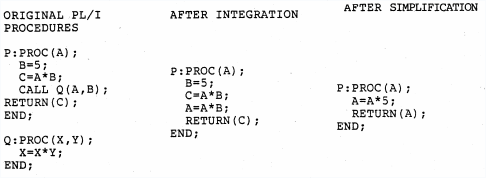
\includegraphics[width=.7\textwidth]{imgs/fig6.png}};

    
\end{frame}

\begin{frame}
    \centering 
    \tikz 
    \node at (current page.center) {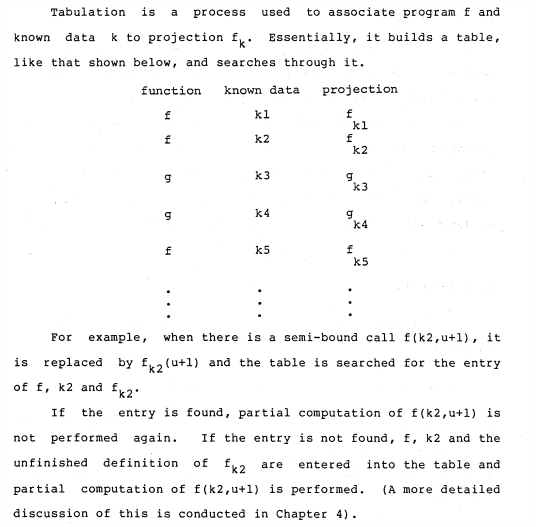
\includegraphics[width=.7\textwidth]{imgs/tabulation.png}};
\end{frame}



\begin{frame}
    \centering 
    \tikz 
    \node at (current page.center) {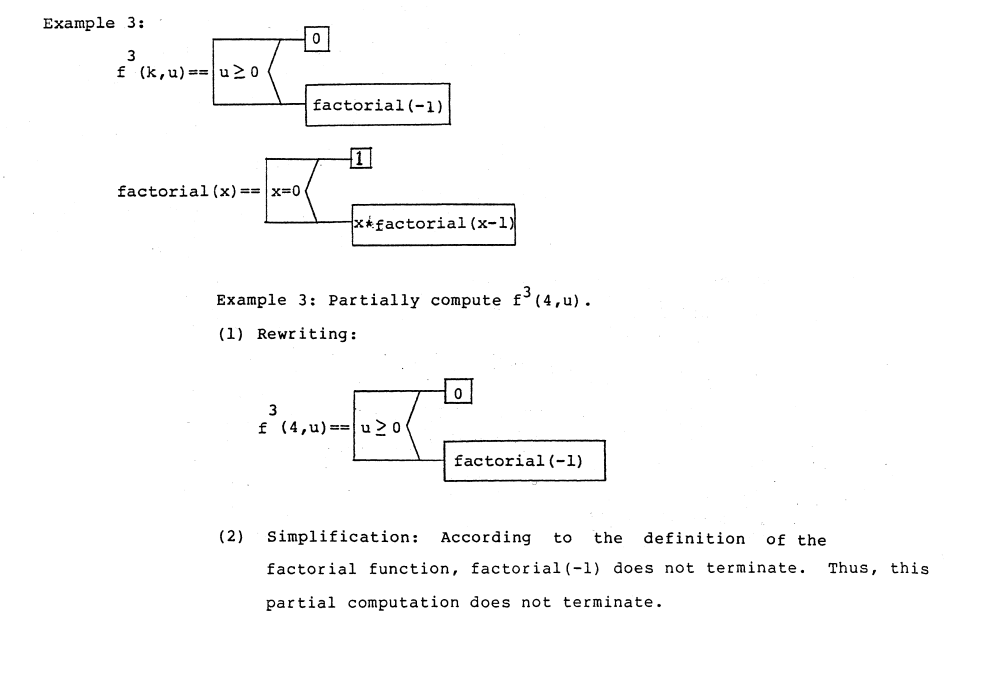
\includegraphics[width=\textwidth]{imgs/notation-fact.png}};
\end{frame}


\begin{frame}
    \centering 
    \tikz 
    \node at (current page.center) {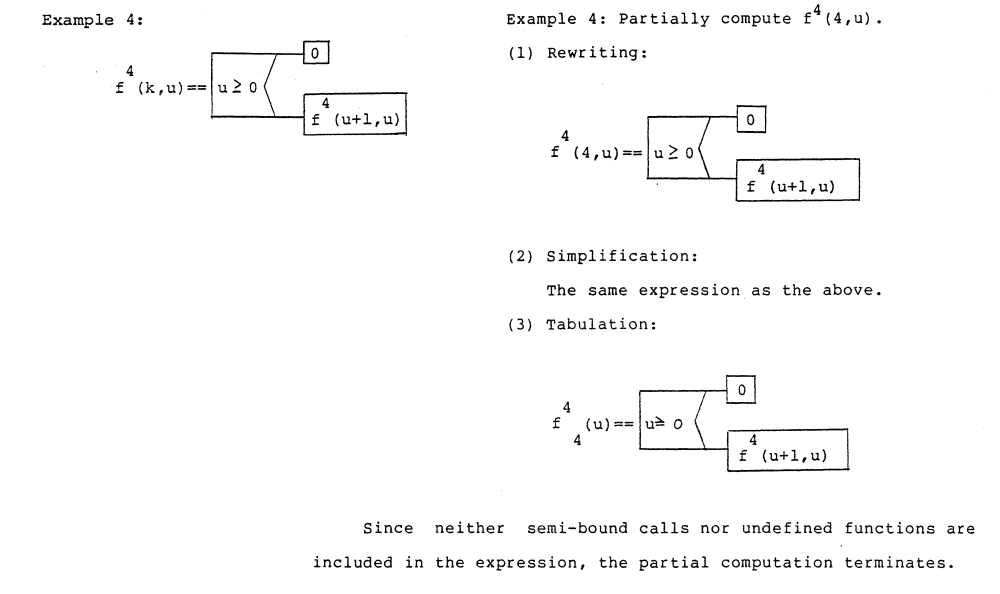
\includegraphics[width=\textwidth]{imgs/notation.png}};
\end{frame}


\begin{frame}
    \centering 
    \tikz 
    \node at (current page.center) {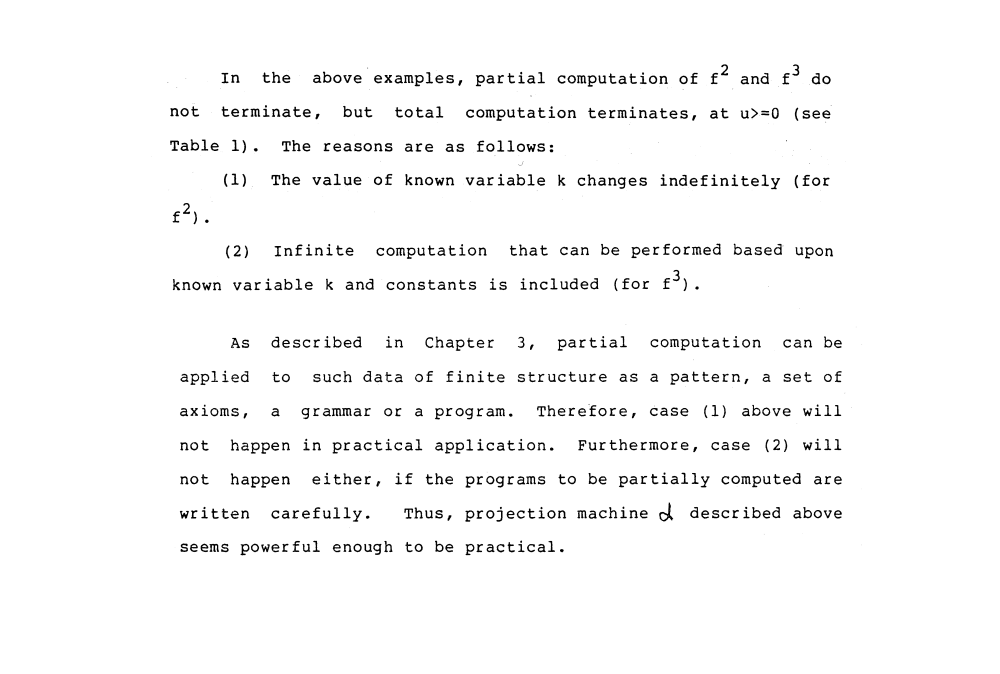
\includegraphics[width=\textwidth]{imgs/notation-concl.png}};
\end{frame}



\begin{frame}[c]
\centering \Large \bf \color{Blue} GraalVM 
\end{frame}

\begin{frame}
    \centering 
    \tikz 
    \node at (current page.center) {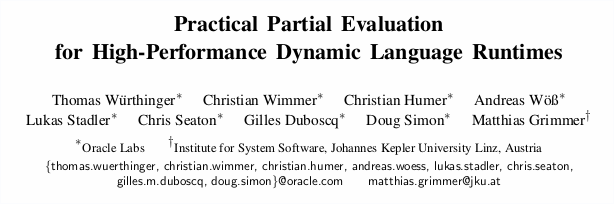
\includegraphics[width=\textwidth]{imgs/truffle.png}};

\end{frame}


\begin{frame}
    \textcolor<2>{lightgray}{
    We implement the language semantics only once in a
simple form: as a \alert<2>{language interpreter} written in a 
managed high-level host language. Optimized compiled code is
\alert<2>{derived from the interpreter using partial evaluation}. This
approach and its obvious benefits were described in 1971
by Y. Futamura, and is known as the \alert<2>{\textit{first Futamura
projection}}. To the best of our knowledge no prior high-
performance language implementation used this approach.
    }
\end{frame}
     
\begin{frame}
\textcolor<2>{lightgray}{
We believe that a simple partial evaluation of a dynamic
language interpreter cannot lead to high-performance compiled code: 
if the \alert<2>{complete semantics} for a language operation are included 
during partial evaluation, the \alert<2>{size of the
compiled code explodes}; if language operations are not included 
during partial evaluation and \alert<2>{remain runtime calls},
\alert<2>{performance is mediocre}. To overcome these inherent problems, 
we write the interpreter in a style that anticipates and
embraces partial evaluation. The \alert<2>{interpreter specializes the
executed instructions}, e.g., collects type information and
profiling information. The compiler \alert<2>{speculates} that the interpreter 
state is stable and creates highly optimized 
and compact machine code. If a speculation turns out to be wrong,
i.e., was too optimistic, execution transfers back to the interpreter. 
The interpreter updates the information, so that the
next partial evaluation is less speculative.
}
\end{frame}

\begin{frame}
    \tikz 
    \node at (current page.center) {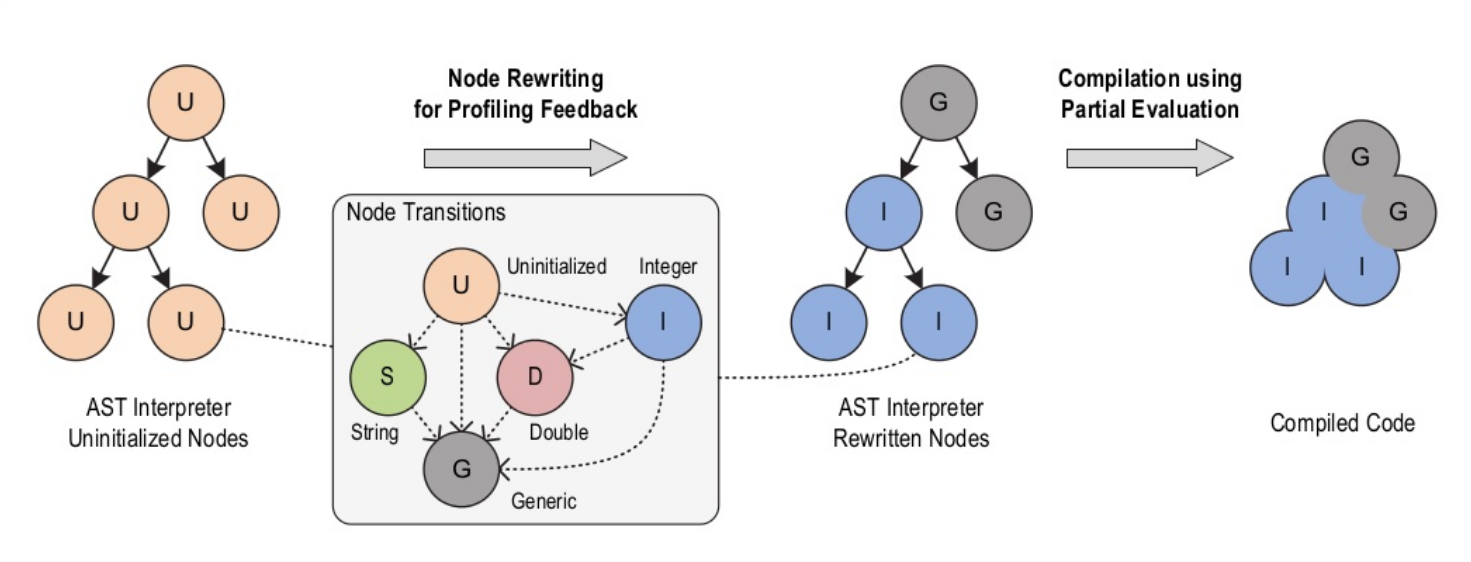
\includegraphics[width=\textwidth]{imgs/onevm.png}};
\end{frame}


\begin{frame}
    \tikz[overlay]
    \node at (6,-.5) {
\includegraphics[width=19cm]{imgs/futamura.png}};
\end{frame}


\begin{frame}[c]{References}
    \begin{itemize}
        \item 
            W\"urthinger et al. 2017
        \item 
            \v Selajev, O. 2018 
            \href{https://gotober.com/2018/sessions/650/graalvm-run-programs-faster-anywhere}{GraalVM: Run Programs Faster Anywhere}
            \textit{GOTO Berlin 2018}

        \item 
            Stuart, T. 2013
            \href{https://codon.com/compilers-for-free}{Compilers for Free}
            \textit{RubyConf 2013}

    \end{itemize}

\end{frame}

\end{document}
    